\chapter{Nutzungsanforderungen}
\label{chapter:user-requirements}

\section{Interview im Kontext}
\label{subsection:IIK}

Das Modul zur Terminvereinbarung der Software Stubegru soll in Bezug auf den
Arbeitsalltag der allgemeinen Studienberatung der Universität Kassel
überarbeitet werden. Dies soll mit Methoden des Human Centered Design umgesetzt
werden. Ein zentraler Bestandteil des Human Centered Design ist der enge und
stetige Austausch mit den Betroffenen des Softwaresystems\cite{hci}. Um den
Änderungsbedarf eines bestehenden Softwaresystems einschätzen zu können wird im
Human Centered Design häufig die Methode des \textit{Interviews im Kontext}
gewählt\cite{contextualDesign}. Diese Methode eignet sich besonders zu Beginn
des Entwicklungsprozesses, da wenig Vorkenntnisse über die eingesetzte Software
und das Umfeld, in dem diese eingesetzt wird, bekannt sein muss. Die
Softwareentwickler können so einen guten Einstieg finden, um einen Überblick zu
gewinnen, welche Funktionen die fertige Software am Ende unterstützen muss.
Auch lässt sich durch ein genaues Beobachten beim Interview herausarbeiten, in
welchem Kontext die Software im tatsächlichen Arbeitsalltag genutzt wird und
welche weiteren Faktoren die Betroffenen der Systeme beeinflussen.

\subsection*{Rahmenbedingungen des Interviews im Kontext}
Als erster Schritt wurde ein Termin für ein Interview im Kontext mit
\ipName\footnote{Aufgrund des Datenschutzes wurde der Name anonymisiert}
vereinbart. \ipName ist einer von drei Mitarbeitenden der allgemeinen
Studienberatung der Universität Kassel. Zu seinen Aufgaben gehört die Betreuung
der Software Stubegru und deren Einsatz in der Abteilung Studium und Lehre.
Seit über sechs Jahren arbeitet \ipName bereits gemeinsam mit Hilfskräften an
dem Aufbau und der Optimierung der Software Stubegru um den täglichen
Arbeitsalltag seines Teams optimal zu unterstützen. Ich habe mich persönlich
mit \ipName in seinem Büro im Campus Center der Universität getroffen. Dort hat
er mir an seinem Schreibtisch gezeigt, wie er mit der alten Version der
Software Beratungstermine erstellen und vergeben kann. \ipName saß vor mir und
hatte Maus und Tastatur in der Hand. Ich saß hinter ihm auf einem Stuhl und
habe auf einem iPad Notizen mitgeschrieben. Für die Dauer von einer Stunde hat
\ipName mir gezeigt, wie er die Software aktuell nutzt, welche Features für ihn
sehr wichtig sind und an welchen Stellen noch Verbesserungspotenzial besteht.

\subsection*{Detaillierter Ablauf des Interviews}
Am Anfang habe ich \ipName gebeten, mir einmal zu zeigen, wie er einen
Beratungstermin in der Software anlegen und vergeben kann. Dies ist der
Workflow, der im Arbeitsalltag am häufigsten vorkommt und daher eine hohe
Priorität im Designprozess hat. \ipName klickte sich durch die verschiedenen
Eingabefelder um einen freien Zeitslot für einen Beratungstermin anzulegen.
Hierbei erwähnte er, dass es ganz wichtig ist, dass Datum und Uhrzeit des
Beratungstermins mit wenigen Klicks über einen \gls{Timepicker} mit der Maus
eingeben werden können. Eine Datumseingabe über die Tastatur würde er nicht
bevorzugen.

\begin{figure}[H]
    \caption{Datepicker im Formular zur Erstellung eines Zeitslots}
    \centering
    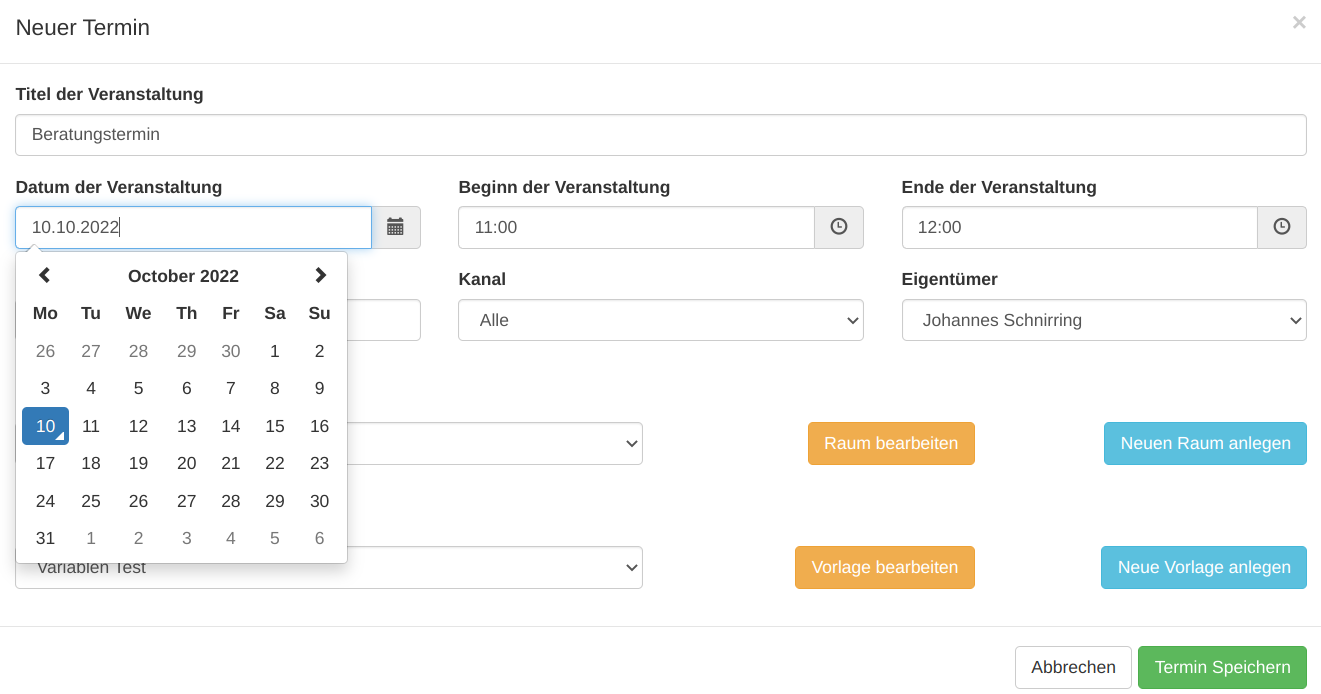
\includegraphics[width=0.9\textwidth]{screen_old_datepicker.png}
\end{figure}

Beim Eintragen mehrere Termine wäre es auch besonders praktisch, dass das zuvor
eingegebene Datum stehen bleibt und direkt ein weiterer Zeitslot für den
gleichen Tag angelegt werden kann, ohne dass er nochmal extra das Datum
auswählen muss. Die meisten weiteren Felder sind Dropdown Menüs, mit wenigen
Elemente. Die Auswahl der richtigen Werte kann \ipName schnell vornehmen. Bei
der Auswahl der verknüpften Räume werden beispielsweise die Räume, die mit
seinem Nutzeraccount verknüpft sind, ganz oben in der Auswahlliste angezeigt.
Da eine Beratung in der Regel in den eigen Räumen stattfindet, ist hier eine
schnelle Auswahl für den Normalfall möglich. In einer Spezialsituation, in der
ein größerer Beratungstermin beispielsweise in einem gemeinsamen Gruppenraum
stattfinden, ist aber auch solch eine Auswahl möglich.

\begin{figure}[H]
    \caption{Dropdown zur Auswahl des Beratungsraums. Der eigene Raum wird immer als oberstes angezeigt}
    \centering
    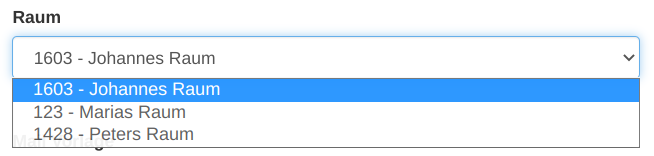
\includegraphics[width=0.9\textwidth]{screen_old_roomdropdown.png}
\end{figure}

Nachdem der Zeitslot für den Termin angelegt ist, wird der entsprechende Tag in
der Kalenderübersicht nun grün hinterlegt. Dies ist ein Zeichen für die
Hilfskräfte der Erstinformation, dass an diesem Tag noch freie Zeitslots
verfügbar sind.

\begin{figure}[H]
    \caption{Kalenderübersicht. Grüne gefärbte Tage zeigen noch freie Zeitslots an. Rot gefärbte Tage weisen auf vergeben Zeitslots hin}
    \centering
    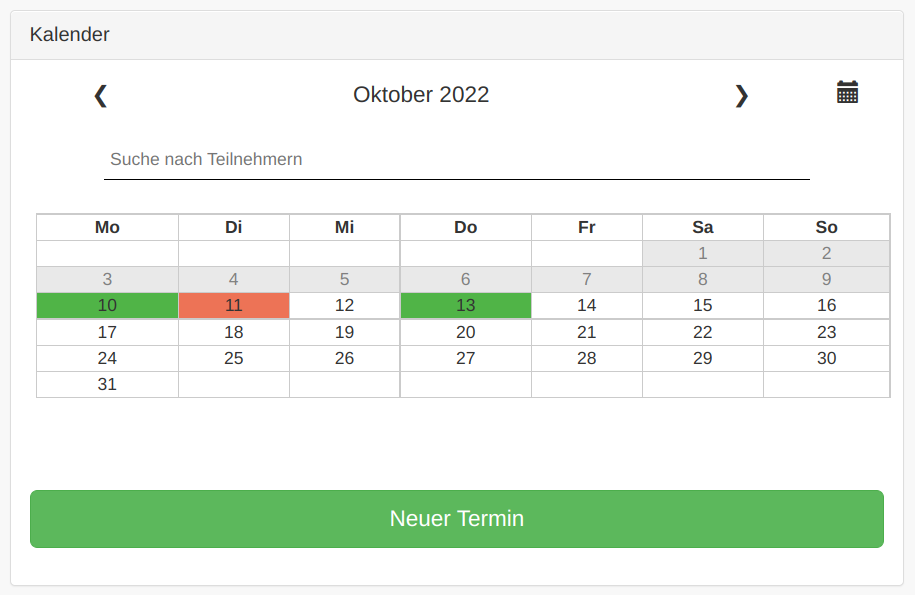
\includegraphics[width=0.9\textwidth]{screen_old_module.png}
\end{figure}

Wenn \ipName den Mauszeiger über den entsprechenden Tag in der Monatsübersicht
bewegt, kann man die genauen Termine mit Informationen über die Uhrzeit, den
zuständigen Beratenden und die Anzahl der freien Plätze sehen. \ipName erklärt
mir, dass die kompakte Monatsansicht mit den farblich hervorgehobenen
Terminslots bereits eine sehr gute Lösung ist, damit die Hilfskräfte auf einen
Blick erfassen können, an welche Tagen sie den Kunden noch Beratungsgespräche
anbieten können. Sobald alle Plätze der Beratungstermine an einem Tag vergeben
sind, wird dieser im Kalender rot markiert. \glqq{}So sehen Hilfskräfte mit
einem Blick sofort, dass sie hier keinen Termin mehr vergeben werden
können\grqq{}, erklärt \ipName \cite{claves}.

\begin{figure}[H]
    \caption{Bewegt man den Mauszeiger über einen Tag, erscheinen weiteren Informationen zu den Zeitslots an diesem Tag}
    \centering
    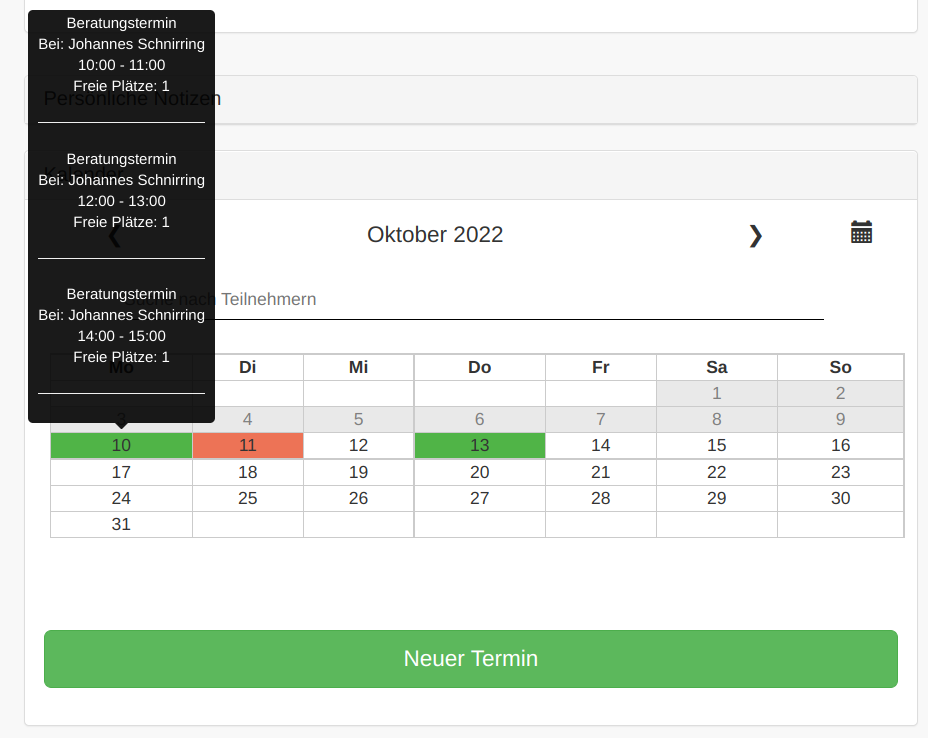
\includegraphics[width=0.9\textwidth]{screen_old_hover.png}
\end{figure}

Soll nun ein Zeitslot tatsächlich vergeben werden, klickt man auf den
entsprechenden Tag in der Monatsansicht und es öffnet sich ein \gls{Modal}.
Dies ist ein Fenster, welches sich über den anderen Bildschirminhalt legt und
dem Nutzer somit deutlich anzeigt, dass hier eine Aktion im neu geöffnet
Fenster notwendig ist. \ipName zeigt mir, wie die Mitarbeitenden der
Erstinformation in diesem Detail-\gls{View} die freien Zeitslots an die
ratsuchenden Personen vergeben können. In einer Liste werden, nach Uhrzeit
sortiert, alle Termine untereinander angezeigt. Neben jedem freien Termin steht
ein Button zum Vergeben dieses Zeitslots zur Verfügung.

\begin{figure}[H]
    \caption{Der Detail-View: Eine Liste mit drei freien Zeitslots}
    \centering
    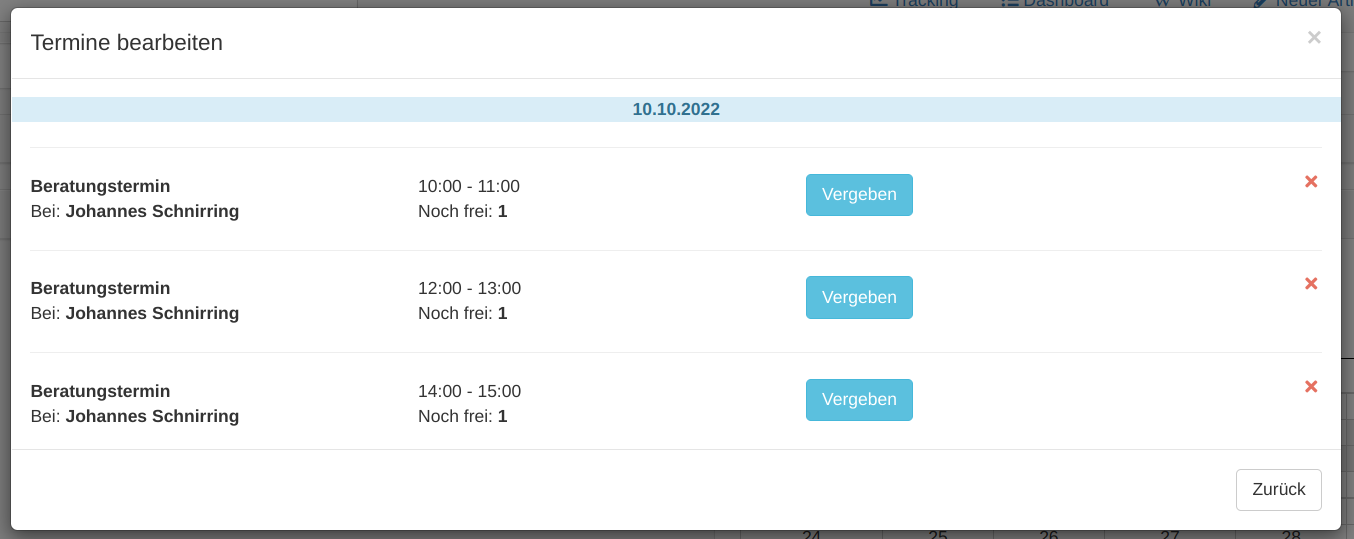
\includegraphics[width=0.9\textwidth]{screen_old_daylist.png}
\end{figure}

\ipName zeigt mir wie eine Hilfskraft der Erstinformation nun einen solchen
Zeitslot vergeben könnte. Nach Klick auf den \textit{Vergabe-Button} klappt ein
Formular auf, indem Name, Kontaktdaten und Anliegen der Ratsuchenden erfasst
werden können.

\begin{figure}[H]
    \caption{Formular zum Vergeben eines Zeitslots an eine ratsuchende Person}
    \centering
    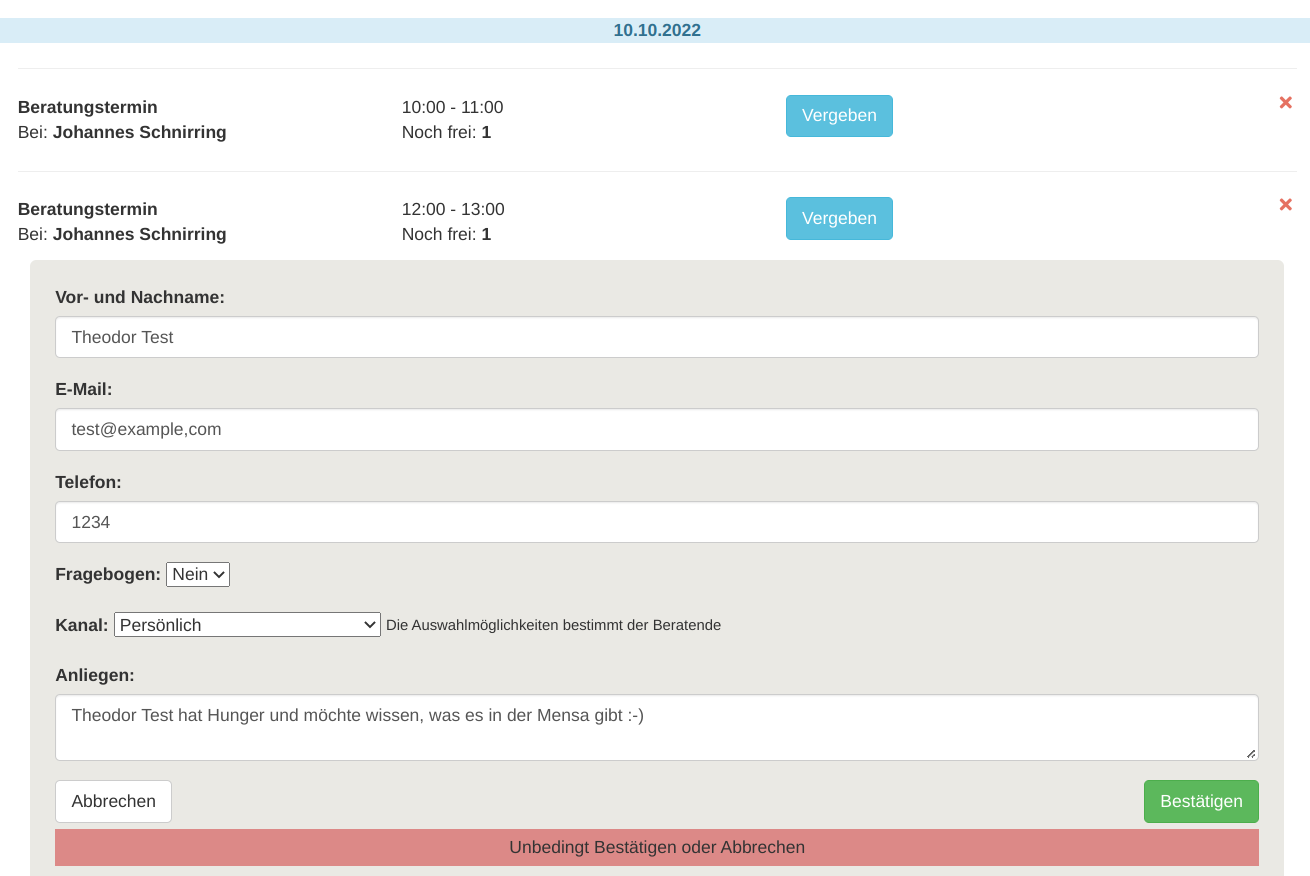
\includegraphics[width=0.9\textwidth]{screen_old_clientdata.png}
\end{figure}

Nachdem alle personenbezogenen Daten korrekt erfasst wurden kann der Termin nun
endgültig gebucht werden. Hierzu klicken die Hilfskräfte auf den Button
\textit{Bestätigen}. \ipName erklärt mir, dass dies ein sehr wichtiger Schritt
ist: Solange eine Mitarbeitender der Erstinformation das Formular zum Erfassen
der persönlichen Daten des Ratsuchenden geöffnet hat, wird dieser Zeitslot mit
einer Sperre versehen. So wird verhindert, dass dieser Zeitslot von einem
Kollegen vergeben werden kann, während man selbst gerade mit dem Ratsuchenden
am Telefon die persönlichen Daten und das Anliegen bespricht. Sollte nach dem
Aufklappen des Formulars der entsprechende Zeitslot doch nicht vergeben werden,
ist es deshalb notwendig, dass die terminvergebende Person auf
\textit{Abbrechen} klickt, um die Sperre dieses Zeitslots aufzuheben und ihn
somit für die Kollegen wieder freizugeben. \ipName betont, dass dieser Schritt
manchmal nicht ganz intuitiv ist, und für die Hilfskräfte daher in
Einführungsschulungen immer besonders hervorgehoben wird. Es wäre allerdings
deutlich schlimmer einen Termin doppelt zu vergeben und somit mindestens einem
Kunden wieder absagen zu müssen, als einen Zeitslot versehentlich zu sperren.

\begin{figure}[H]
    \caption{Detail-View: Ein Zeitslot wurde nun vergeben und ist für den entsprechenden Kunden reserviert. Hilfskräfte können nur den Namen des Ratsuchenden einsehen}
    \centering
    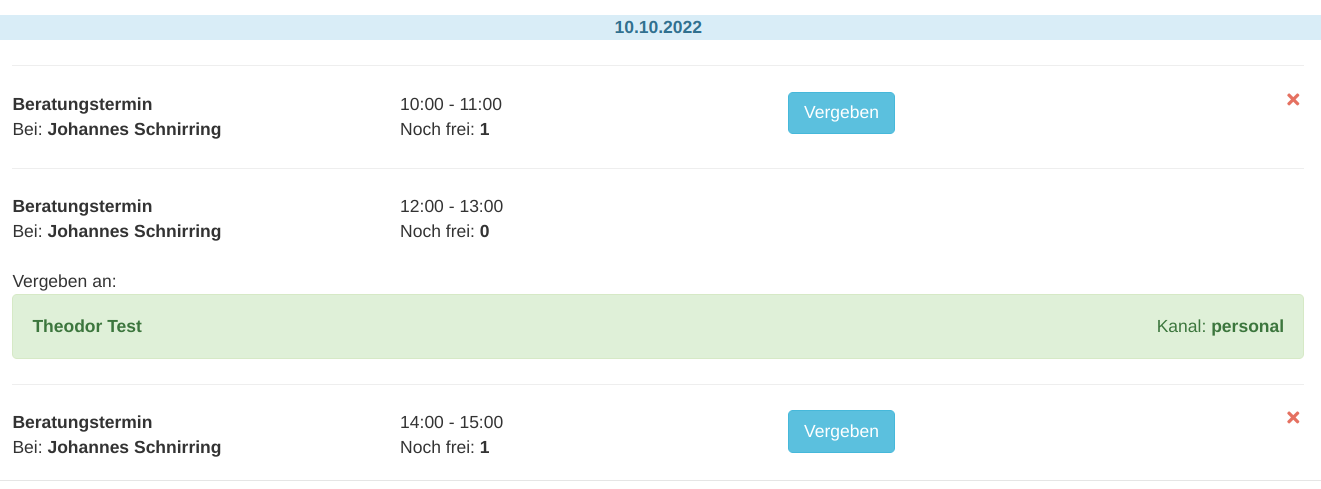
\includegraphics[width=0.9\textwidth]{screen_old_assigned_hiwi.png}
\end{figure}

Ist der Termin nun erfolgreich vergeben, können alle Nutzenden der Software
einsehen an welche Person dieser Termin vergeben wurde. Meldet sich ein
Ratsuchender beispielsweise einige Tage später noch einmal bei der
Erstinformation und möchte wissen, wann sein Beratungstermin stattfindet,
können die Mitarbeitenden der Erstinformation diese Auskunft aus der Software
ablesen. Aus Datenschutzgründen können allerdings keine weiteren
personenbezogenen Daten des Beratungstermins ausgelesen werden. Lediglich der
Studienberatende, bei dem der Termin stattfindet, bekommt beim Aufruf des
Detail-Views weitere Details wie Kontaktdaten und Anliegen der ratsuchenden
Person angezeigt.

\begin{figure}[H]
    \caption{Detail-View: Der verantwortliche Beratende kann weitere personenbezogene Details einsehen}
    \centering
    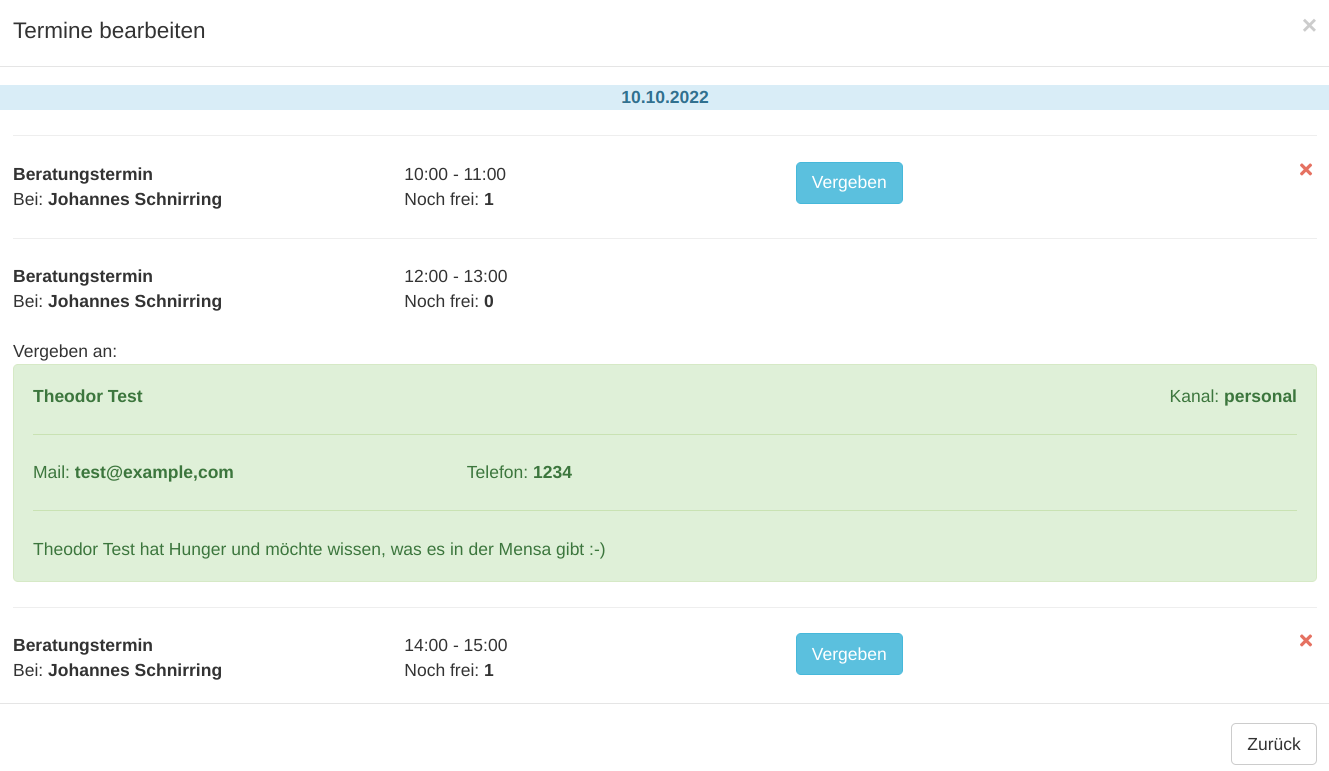
\includegraphics[width=0.9\textwidth]{screen_old_assigned.png}
\end{figure}

\ipName hat nun den zweistufigen Workflow zur Terminvergabe einmal komplett
durchgespielt und mich auf viele Details hingewiesen. Während \ipName mir
gezeigt und erzählt hat, wie die Terminvergabe in der aktuellen Softwareversion
abläuft, habe ich in Stichworten mitgeschrieben, welche Bemerkungen und
Auffälligkeiten er besonders betont hat.

\section{Auswertung des Interviews}

Während bisher der detaillierte Ablauf des Interviews geschildert wurde, sollen
im Folgenden die wesentlichen Kernaspekte nochmals zusammengefasst werden, die
während des Interviews notiert wurden. Das Augenmerk liegt hierbei auf
Beobachtungen, die Konsequenzen für den Designprozess des neuen Kalendermoduls
zur Terminvergabe hervorbringen.

\subsection*{Methode der Auswertung}
Während dem Interview habe ich mir alle relevant erscheinenden Aussagen von
\ipName auf einem iPad notiert. Wurden im weiteren Gesprächsverlauf noch
ergänzenden Informationen zu den einzelnen Punkten deutlich, habe ich diese in
den Notizen stichpunktartig an die entsprechenden Themen angefügt. Im Nachgang
des Interviews mussten diese Notizen nun sorgfältig analysiert und ausgewertet
werden. Hierzu bin ich die einzelnen Themen durchgegangen und habe die
entsprechenden Ansichten und Klickpfade in der Software nochmals nachgespielt.
In einem neuen Dokument habe ich nun die herausgearbeiteten Problematiken
zusammengefasst um die zu Grunde liegenden Zusammenhänge klarzustellen und zu
spezifizieren. Dies entspricht dem zweiten Schritt
\textit{Nutzungsanforderungen spezifizieren} im iterativen Design Zyklus des
Human Centered Design nach ISO 9241\cite{ISO9241}.

\subsection*{Spannende Erkenntnisse}
\label{subsection:SpannendeErkenntnisse}

Das Interview im Kontext hat viele spannende Beobachtungen geliefert, die hier
nicht alle detailliert ausgeführt werden können. Daher sollen im Folgenden nun
drei verschiedene Themen exemplarisch vorgestellt werden, die während des
Interviews aufgefallen sind. Im weiteren Verlauf dieser Arbeit wird in den
unterschiedlichen Phasen des Gestaltungsprozesses immer wieder auf diese Themen
Bezug genommen.

\subsubsection{Kompakte Monatsübersicht}
In der alten Softwareversion, die an der Uni Kassel bisher zum Einsatz kam,
werden alle freien und vergeben Zeitslots der Beratungstermine in einer
tabellarischen Monatsansicht dargestellt.

\begin{figure}[H]
    \caption{Tabellarische Ansicht der Zeitslots mit Einfärbungen der einzelnen Tage}
    \centering
    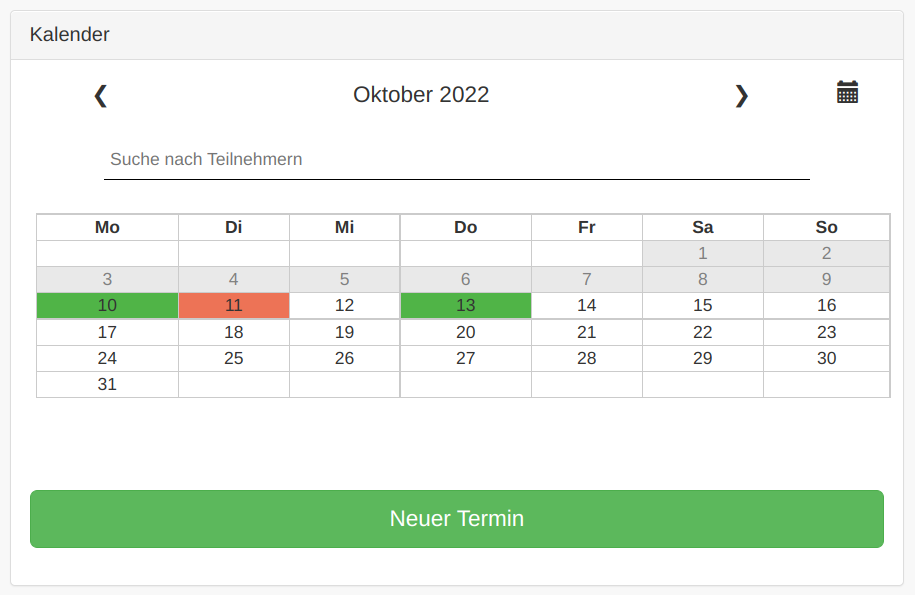
\includegraphics[width=0.9\textwidth]{screen_old_module.png}
\end{figure}

Durch die farblichen Markierungen der einzelnen Tage können Nutzenden auf einen
Blick erfassen, ob an diesem Tag Beratungsslots eingetragen wurden und ob unter
den eingetragenen Zeitslots noch freie Termine vorhanden sind. Ein grün
markierter Tag bedeutet, dass an diesem Tag noch mindestens ein freier
Beratungsslot vorhanden ist. Ein rot markierter Tag bedeutet, dass an diesem
Tag Beratungstermine stattfinden, diese allerdings bereits alle an ratsuchende
Personen vergeben sind. In der überarbeiteten Version der Stubegru Software,
die in Zusammenarbeit mit der Hochschule Bremen entstanden ist, wurde diese
kompakte tabellarische Übersicht durch eine größere umfangreiche Ansicht
ausgetauscht, die durch die Bibliothek \gls{fullcalendar} bereitgestellt wird.

\begin{figure}[H]
    \caption{Monatsübersicht der Beratungstermine in der \textit{Bremer Version}}
    \centering
    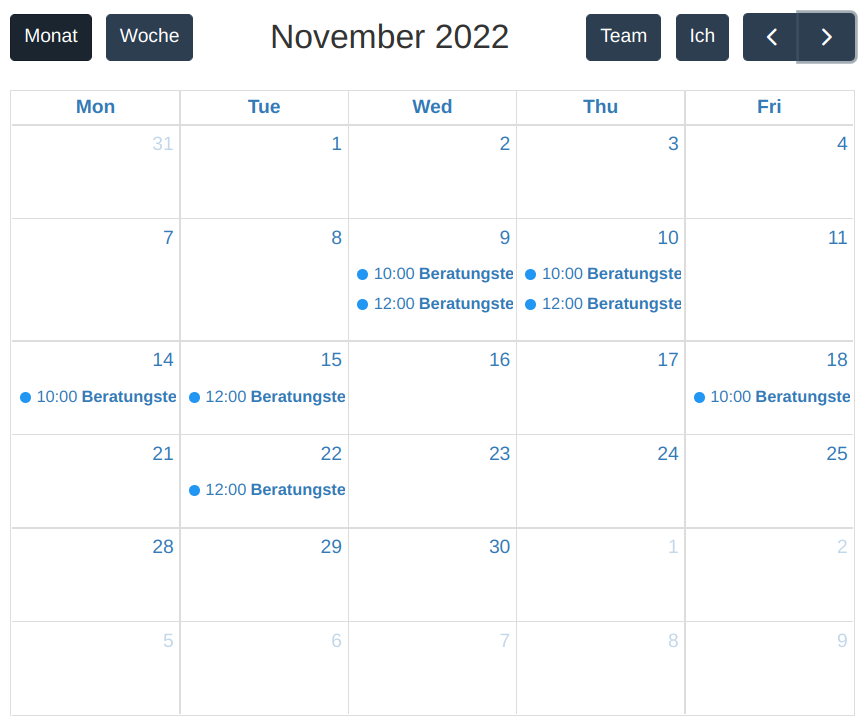
\includegraphics[width=0.9\textwidth]{screen_bremen_month_view.png}
\end{figure}

Diese neue Ansicht ermöglicht auf den ersten Blick zu sehen, zu welcher Uhrzeit
die Termine stattfinden und einzelne Termine aus der Monatsübersicht direkt
anzuklicken. Allerdings bietet diese Ansicht keine Möglichkeit, Tage je nach
freien Plätzen rot oder grün darzustellen. Dies ist jedoch ein wichtiges
Feature für die zweistufige Terminvergabe an der zentralen Studienberatung der
Universität Kassel. An dieser Stelle braucht es eine Idee um den Hilfskräften
der Erstinformation auf den ersten Blick anzuzeigen, ob sie an diesem Tag noch
freie Terminslots vergeben können.

\subsubsection{Suche nach Teilnehmern}
Manchmal kommt es vor, dass Ratsuchende, die bereits einen Beratungstermin
vereinbart haben, nochmals in Kontakt mit der Erstinformation treten, um
weitere Fragen zum Termin zu stellen. Auch kommt es vor, dass das genaue Datum
oder die Uhrzeit vergessen wurden. In diesem Fall sollen die Hilfskräfte der
Erstinformation möglichst schnell Auskunft über die angefragten Details geben
können. Hierfür immer alle vergebenen Beratungstermine manuell durchzulesen,
ist zeitlich ein großer Aufwand. Es braucht also ein Feature, sodass die
Mitarbeitenden der Erstinformationen direkt nach Terminen und weiteren
organisatorischen Daten dieser Termine suchen können. Wenn Ratsuchende
beispielsweise am Telefon ihren Namen nennen, werden sie manchmal nicht
einwandfrei verstanden. Ein Suche nach Teilnehmernamen der Termine sollte also
auch funktionieren, wenn der Name nicht exakt in der gleichen Schreibweise
eingegeben wird, wie er im Datensatz des Beratungstermins in der Datenbank
hinterlegt ist.

\subsubsection{Darstellung der Telefonnummern}
In der Regel wird bei einer Terminvergabe die Telefonnummer der ratsuchenden
Person erfasst. Der zuständige Studienberatende kann den Datensatz bei Bedarf
aufrufen und diese Telefonnummer einsehen. Dies passiert in der Regel, wenn der
Beratende vor einem Beratungstermin nochmals telefonisch Details mit der
ratsuchenden Person abklären möchte. Der Berater wählt also die angezeigte
Telefonnummer in seinem Telefon. Während des Interviews im Kontext zeigte sich,
dass die Eingabe längerer Telefonnummern manchmal Fehler mit sich bringt, da
Ziffern vertauscht oder vergessen werden. Den Beratenden wäre hier eine
wertvolle Hilfe an die Hand gegeben, wenn eine Darstellung langer
Telefonnummern möglich wäre, die ein direktes und intuitives Eintippen in die
Telefontastatur erleichtert.

\section{Gestaltungslösungen entwickeln}

Nachdem nun die Problematiken und Herausforderungen des neuen Softwaremoduls
verdeutlicht wurden, sollen im nächsten Schritt konkrete Ideen entwickelt
werden, wie die erkannten Problematiken und Anforderungen in der Praxis
umgesetzt werden können. Alan Dix betitelt diese Phase in \textit{Human
    Computer Interaction} als \textit{Requirements specification} und betont, dass
der Fokus in diesem Schritt darauf liegt, die notwendigen Funktionalitäten und
Features der Software grob zu beschreiben. Von besonderer Bedeutung in diesem
Schritt des Designzyklus sind Zusammenhänge und Abhängigkeiten zwischen
einzelnen Komponenten. Exakte Implementierungsdetails hingegen sind in dieser
Phase noch nicht von großer Bedeutung und sollten erst im nächste Schritt
genauer betrachtet werden\cite{hci}.

\subsection*{Methode der Erarbeitung}
Durch die Auswertung des Interviews im Kontext sind Nutzungsanforderungen an
das neue Modul zur Terminvereinbarung entstanden. Um diese lose formulierten
Nutzungsanforderungen später implementieren zu können, werden sie in diesem
Schritt weiter konkretisiert. Es sollen erste Ideen entstehen, wie die
Bedürfnisse der Nutzenden durch einzelne Komponenten der Software umgesetzt
werden können. In diesem Fall wird mit Skizzen der einzelnen \glspl{View} und
Formulare gearbeitet. Für jedes Szenario, dass Nutzende beim späteren Verwenden
der Software durchlaufen, wird eine Skizze erstellt. Durch Markierungen und
Notizen an der Skizze werden die Funktionen und Beziehungen der Elemente
definiert.

\subsubsection{Kompakte Monatsübersicht}

Die Übersicht aller Termine eines Monats ist die Ansicht, die Nutzende beim
Aufruf der Software als erstes sehen. Dies soll auch in der neuen
Softwareversion erhalten bleiben: Den größten Raum nimmt die tabellarische
Ansicht der einzelnen Tage des Monats ein. In den einzelnen Feldern werden
Terminslots, nach Uhrzeit sortiert, aufgelistet. Neben der Uhrzeit des Termins
wird der Titel eines jeden Termins angezeigt. Die einzelnen Termine werden
farblich entweder grün oder rot eingefärbt, um auf den ersten Blick zu
kennzeichnen, ob es sich um einen freien Terminslot (grün) oder um einen
bereits vergebene Termin (rot) handelt. Wenn an einem Tag viele Zeitslots
angelegt werden, wird das Feld für diesen Tag automatisch größer, sodass alle
Termine Platz finden. Sollten an jedem Tag sehr viel Termine angelegt werden,
könnte die tabellarische Monatsansicht so lang werden, dass sie unter Umständen
nicht mehr vollständig auf den Bildschirm passt. Dies wäre unpraktisch, da dann
nicht mehr alle Termine eines Monats auf einen Blick erfasst werden könnten. In
der Phase der Evaluation sollte Diese Problematik berücksichtigt werden und
eine Abschätzung getroffen werden, wie viele Termine im praktische Einsatz
tatsächlich pro Tag angelegt werden.

\begin{figure}[H]
    \caption{Monatsübersicht der Beratungstermine mit farblichen Markierungen}
    \centering
    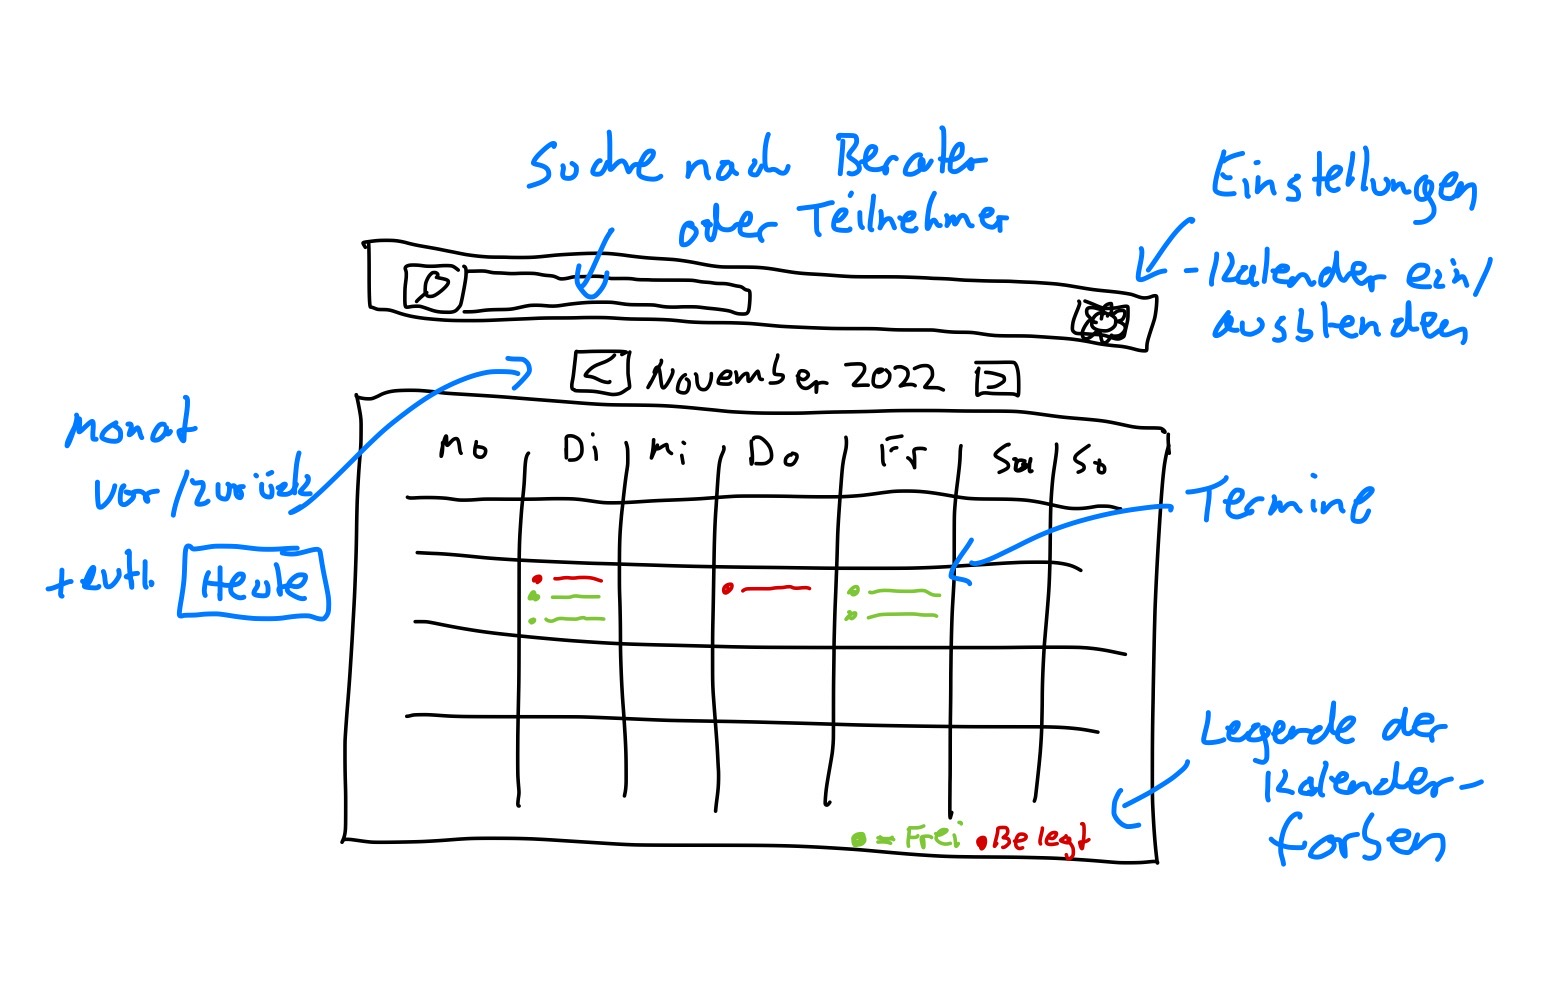
\includegraphics[width=0.9\textwidth]{doodle_month_view.jpeg}
\end{figure}

Über der tabellarischen Ansicht der Tage befindet sich eine horizontale Leiste, die den aktuell angezeigten Monat betitelt und Kontrollelemente beinhaltet um in den vorherigen bzw. nächsten Monat zu wechseln. Über der Leiste mit dem Monat befindet sich eine weitere Kontrollleiste. Diese enthält einen Button um einen neuen Termin anzulegen. Dieser Button sollte nur für Nutzeraccounts von Beratenden sichtbar sein. Hilfskräfte der Erstinformation sollen Zeitslots nur vergeben, aber nicht selbst anlegen können. Daneben befindet sich eine Suchleiste um schnell nach Namen von ratsuchenden Personen suchen zu können. Ganz rechts gibt es schließlich noch einen Button um weitere Einstellungen vorzunehmen. Durch einen Klick auf diesen Button mit dem Zahnrad Symbol soll ein Dropdown-Menü aufklappen, indem Filter für die Ansicht der Termine gesetzt werden können.

\begin{figure}[H]
    \caption{Filtereinstellungen der Kalenderansicht. Das Dropdown Menü öffnet sich durch Klick auf den Zahnrad Button}
    \centering
    \includegraphics[width=0.9\textwidth]{example-image-a}
\end{figure}

In diesem Menü kann über Toggles eingestellt werden, ob nur eigene Termine oder
auch fremde Termine in der Monatsansicht dargestellt werden sollen. Mit
\textit{eigenen Terminen} sind Termine gemeint, die den eigenen Benutzeraccount
als zuständigen Beratenden hinterlegt haben. Außerdem kann ein Filter gesetzt
werden um ausschließlich freie Termine anzuzeigen. Dies kann besonders für
Hilfskräfte bei der Vergabe freier Termine relevant sein, da bereits vergebene
Termine in diesem Fall irrelevante Informationen sind, die von freien Zeitslots
ablenken.

\subsubsection{Suche nach Teilnehmern}

Die Suchfunktion ist ein weiterer Aspekt, dem in dieser Ausarbeitung besonderer
Aufmerksamkeit gewidmet ist. Über das Freitextfeld in der oberen Kontrollleiste
können Nutzende nach Namen von Ratsuchenden suchen, an die bereits Termine
vergeben wurden. Tippt man einige Buchstaben in das Suchfeld ein, klappt eine
Box mit Ergebnisvorschlägen unter der Suchleiste auf und schiebt den restlichen
Inhalt (die tabellarische Monatsansicht) nach unten. In dieser Box werden zur
Suchanfrage passende Termine dargestellt. Für jeden Termin wird in einer Zeile
der Titel, der Name des Ratsuchenden, der Name des Beratenden sowie Datum und
Uhrzeit aufgelistet. Neben jedem Datensatz erscheint ein Button mit einem
Augensymbol. Durch einen Klick darauf wird der entsprechende Termin in der
Detailansicht geöffnet.

\begin{figure}[H]
    \caption{Suche nach Terminen eines Ratsuchenden mit Ergebnisliste}
    \centering
    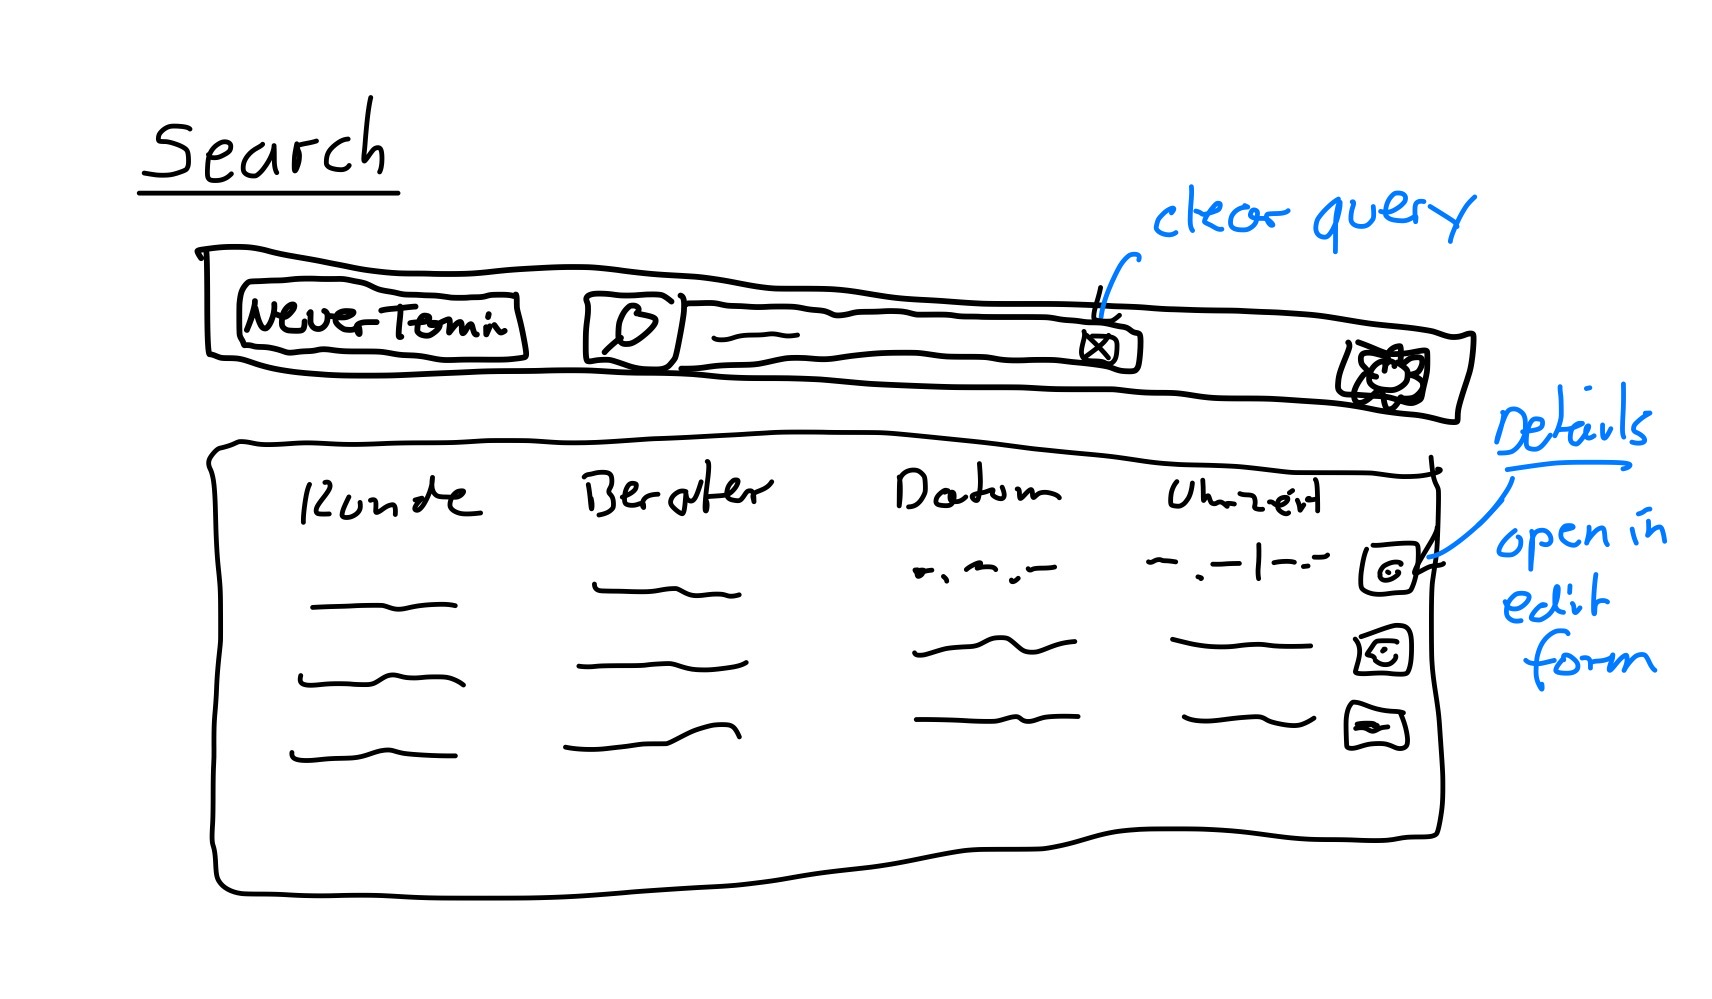
\includegraphics[width=0.9\textwidth]{doodle_search_view.jpeg}
\end{figure}

Wichtig für die Suchfunktion ist, dass passende Ergebnisse auch angezeigt
werden, wenn die Eingabe in der Suchleiste eventuell Fehler enthält oder noch
nicht vollständig ist. Durch solche automatischen Ergebnisvorschläge wird das
Suchen für die Nutzenden erleichtert und Fehlerquellen minimiert. Dadurch, dass
Nutzende schon während dem Tippen der ersten Buchstaben ein aktives und
konstruktives Feedback erhalten, fühlt sich die Nutzung der Software
dynamischer und flüssiger an\cite{autoCompletion}. Wenn Mitarbeitende der
Erstinformation ihre Kunden am Telefon beispielsweise nicht ganz genau
verstehen, können sie mit diesen automatischen Ergebnisvorschlägen trotzdem den
passenden Termin finden. Allerdings muss bei solchen automatisierten
Vorschlägen darauf geachtet werden, dass nicht zu viele unnötige oder
unpassende Vorschläge angezeigt werden. Diese würde Nutzende von den eigentlich
gesuchten Ergebnissen ablenken und sich somit nachteilig auf die
User-Experience auswirken\cite{autosuggModeration}.

\subsubsection{Darstellung der Telefonnummern}

Durch einen Klick auf den Termin in der Monatsübersicht öffnet sich die
Detailansicht des zugehörigen Termins und weitere Eigenschaften des Datensatzes
werden angezeigt. Alternativ kann ein Termin auch über die Suchfunktion
gefunden und dann in der Detailansicht aufgerufen werden. In dieser Ansicht
können Nutzeraccounts mit der entsprechenden Berechtigung nochmals Details des
Termins bearbeiten oder den Termin löschen.

\begin{figure}[H]
    \caption{Detailansicht eines Termins, der bereits an eine ratsuchende Person vergeben wurde}
    \centering
    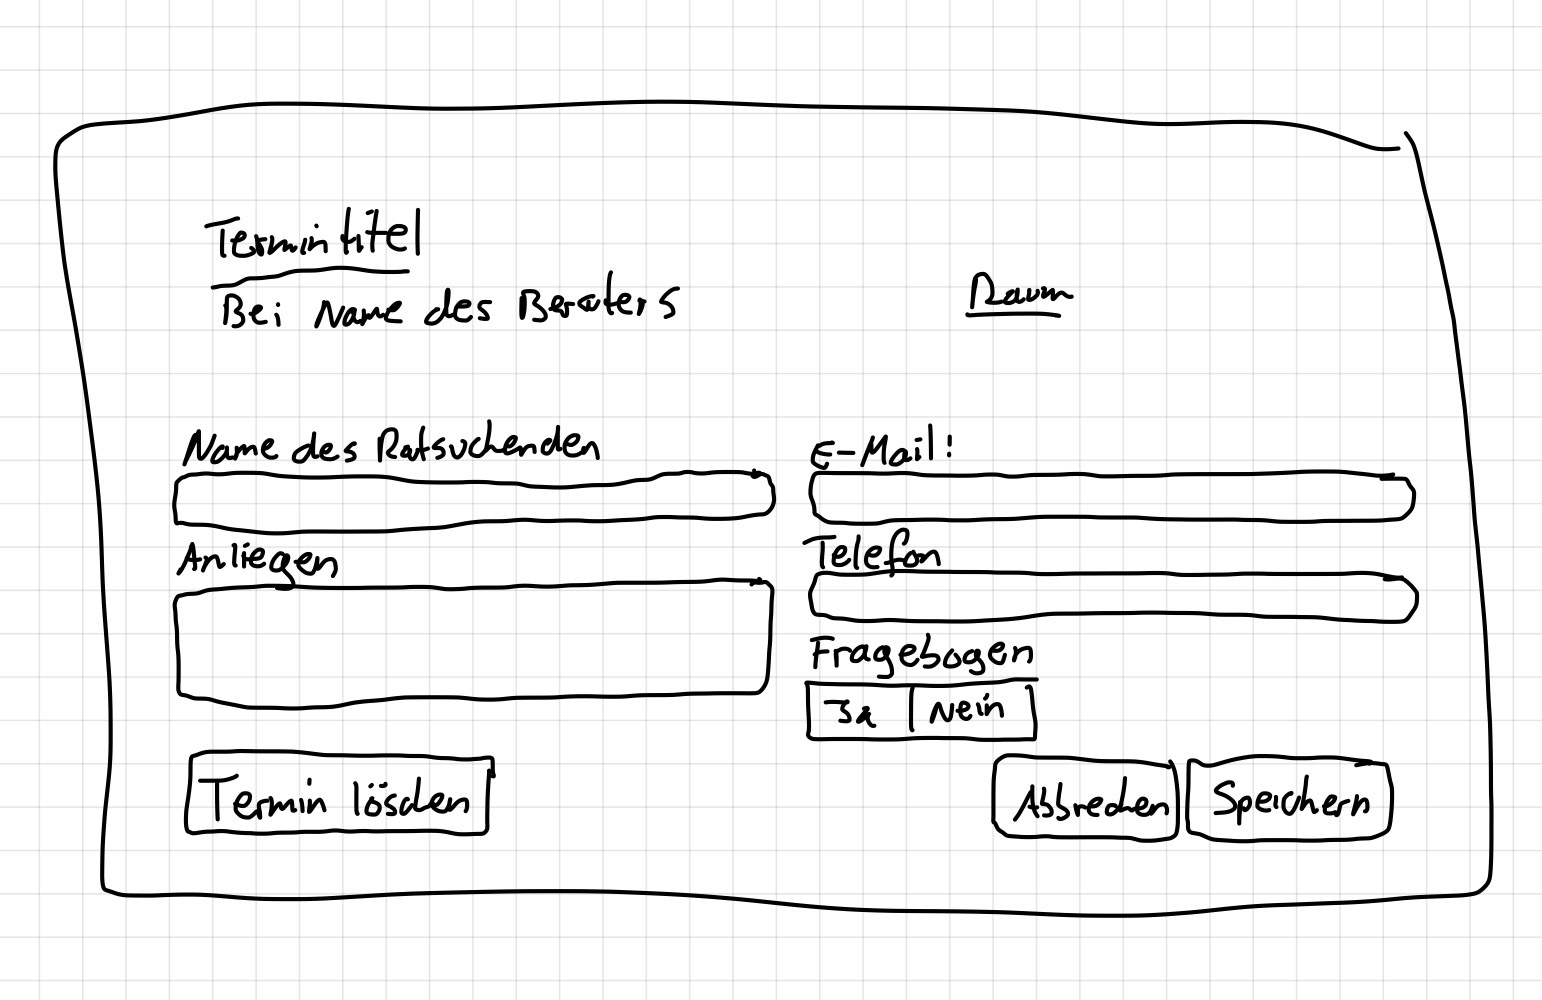
\includegraphics[width=0.9\textwidth]{doodle_client_details.jpeg}
\end{figure}

Wenn Beratende nach der Vereinbarung eines Termins nochmals auf telefonischem
Weg Absprachen oder Vorgespräche mit den Ratsuchenden erledigen möchten, können
sie die Telefonnummer der entsprechenden Person in der Detailansicht eines
Beratungstermins einsehen. Die Beobachtung des Nutzungsverhaltens während des
Interviews im Kontext hat gezeigt, dass es umständlich ist, lange
Telefonnummern zu erkennen und korrekt in die Tastatur des Telefons einzugeben.
Im Gespräch mit \ipName kam der Wunsch auf, Telefonnummern an dieser Stelle so
zu formatieren, dass sie intuitiver erfasst und abgetippt werden können. Der
Standard für das Formatieren von Telefonnummern in Deutschland wird durch DIN
5008 geregelt. Diese Norm beschäftigt sich mit Formatierungsstandards für
Briefe und Anschreiben. Hier wird das Trennen der Vorwahl vom Rest der Nummer
durch ein Leerzeichen vorgeschrieben. Weitere Formatierung, wie beispielsweise
das Aufteilen der Ziffern in kleinere Blöcke wird hier nicht
thematisiert\cite{din5008}.

\begin{figure}[H]
    \caption{So werden nationale Festnetz- und Mobilfunknummern nach DIN 5008 richtig geschrieben. Quelle: \cite{phoneFormatBlog}}
    \centering
    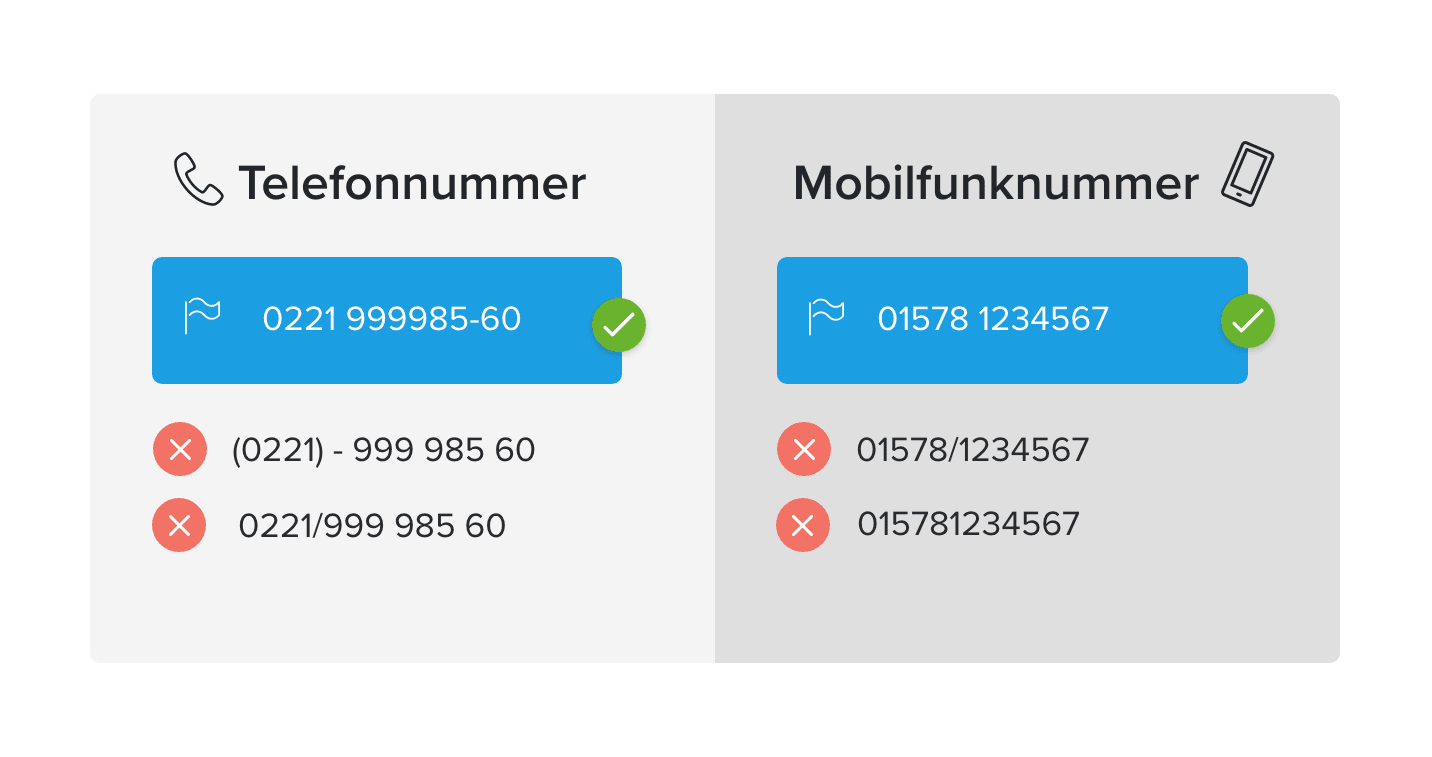
\includegraphics[width=0.9\textwidth]{grafik-telefonnummer-national.png}
\end{figure}

Wissenschaftliche Untersuchungen zeigen, dass das Eingeben und Ablesen von
Telefonnummern in Interaktion mit den entsprechenden Maschinen ein relevantes
Detail ist. Dieser Prozess sollte durch die technischen Systeme möglichst
intuitiv und nutzerfreundlich gestaltet werden\cite{humCompPhoneNumbers}. Eine
Unterteilung der Ziffern in kleinere Blöcke, von beispielsweise vier Ziffern
pro Block, erhört die Lesbarkeit deutlich und ermöglicht es dem menschlichen
Gehirn einen Ziffernblock in einem Blick direkt zu erfassen und auf die
Telefontastatur zu
übertragen\cite{phoneFormatBlog}\cite{numberRecognition}\cite{numberRepres}.